\chapter{Aрхитектура} \label{Architecture}

\section{Организација пакета}

\begin{figure}[htb!]
\begin{center}
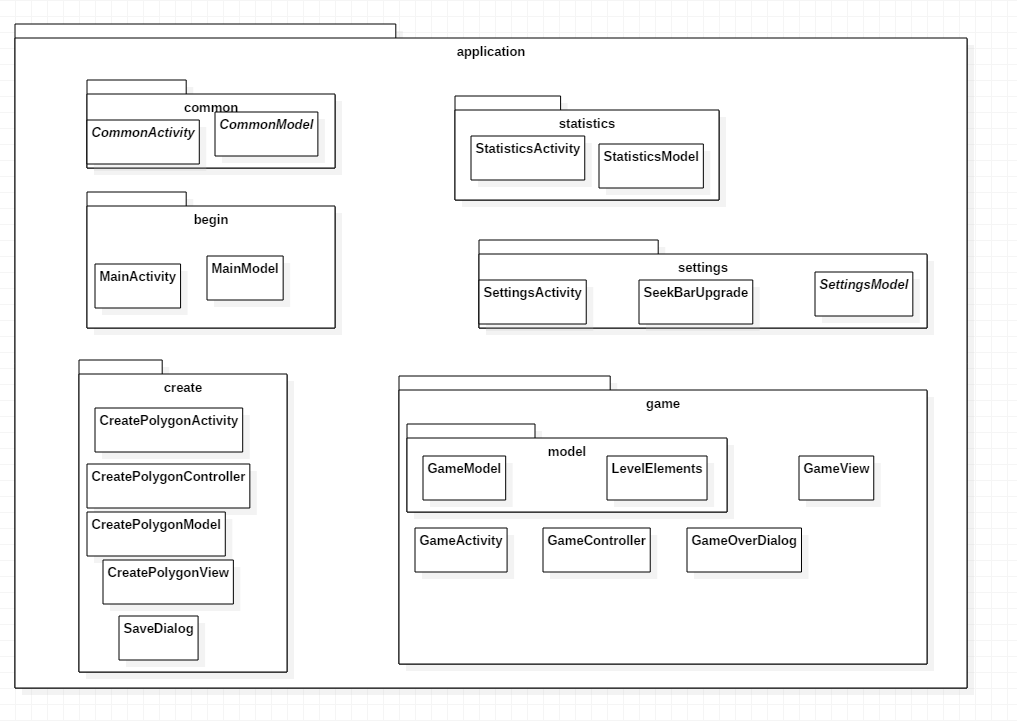
\includegraphics[scale=.7]{pictures/UML/package/application}
\caption{Организација класа по пакетима (application пакет)}\label{fig:umlPackageApp}
\end{center}
\end{figure}

\begin{figure}[htb!]
\begin{center}
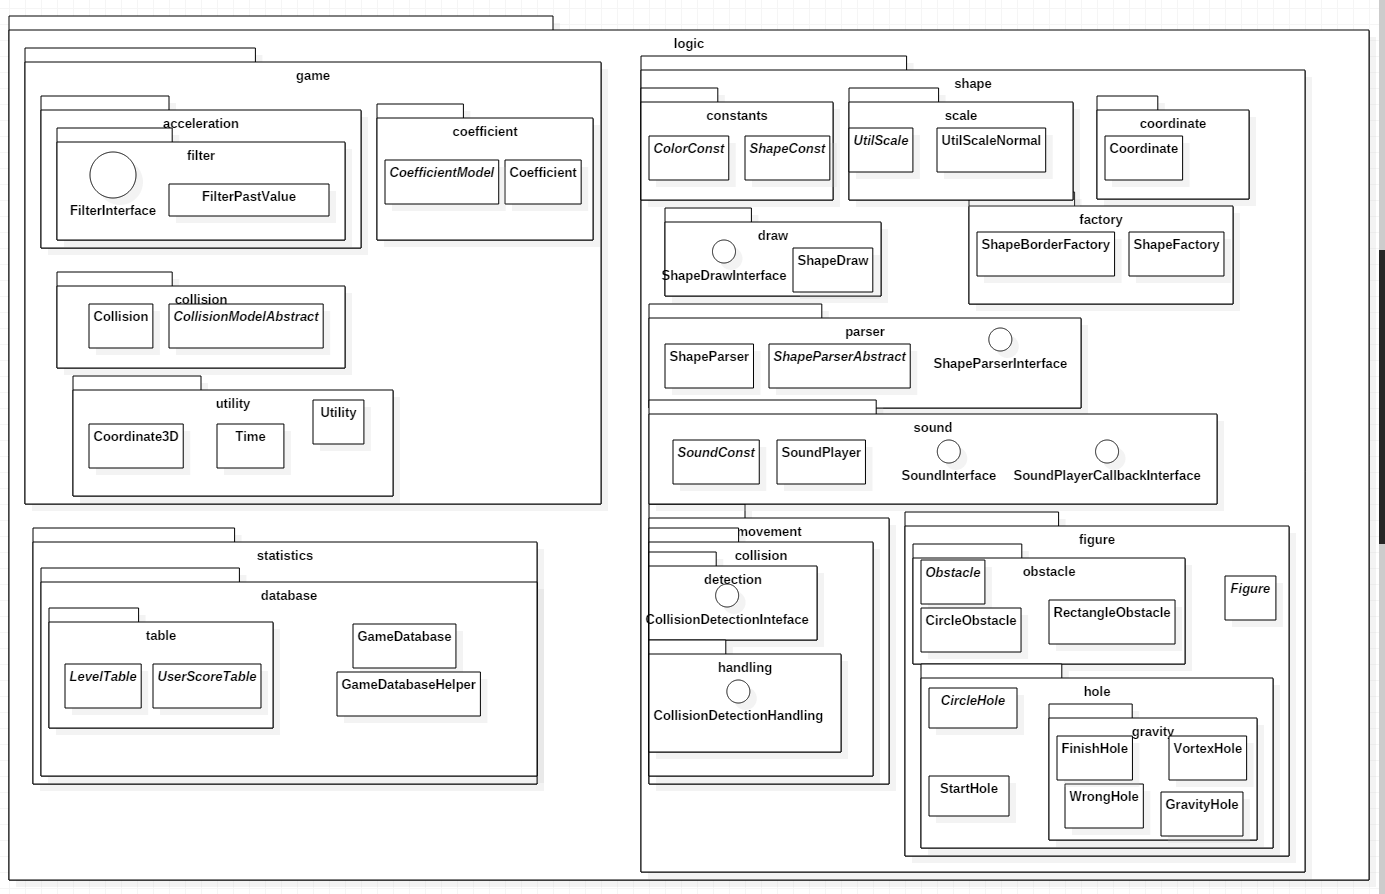
\includegraphics[scale=.6]{pictures/UML/package/logic}
\caption{Организација класа по пакетима (logic пакет)}\label{fig:umlPackageLog}
\end{center}
\end{figure}

Читав java код је организован тако да се налази унутар пакета \emph{com.example.popina.projekat} и то у два потпакета. Код који је везан за MVC преглед и Android део налази се у applicatiоn потпакету (слика \ref{fig:umlPackageApp}). Код који је везан за логику игре (база података, како се праве фигуре, парсира...) налази се у потпакету logic (\ref{fig:umlPackageLog}).